\newpage

\section{Reporting}
Besides logs that the different features and services have, three different reporting tools can be found in the reporting tab on the managing page for the firewall. The reporting tab in \opnsense\ contains a total of five different tabs. Those are:
\begin{itemize}
    \item Health - Gives you information about the firewall, such as the amount of traffic that is going through each of the interfaces. It is also possible to get information about the system, like how much of the RAM or CPU is used, how many states are known by the firewall, and CPU temperature if the hardware supports it (Not supported in our case, since we are using a virtual hypervisor). The information displayed here is not ''live''. You need to update the page to get updated information. An example can be seen in figure \ref{opnsense:reporting_health}. The data that is collected is called RRD (Round Robin Data). The displayed data can be exported to a \cmd{.csv} using the \cmd{Show Tables} function on the top right side of the screen.
    \item Insight - This is the local collector for the NetFlow information, and it displays it in pie charts. 
    \item NetFlow - Create packages that contain information about the different data streams. The package contains:
    \begin{itemize}
        \item IP (source and destination).
        \item Port (source and destination).
        \item Amount of bytes and packages for the stream.
        \item Time of the stream.
        \item Ingress and egress interface\footnote{Ingress = traffic to or from the firewall. Egress = traffic passing through the firewall}.
        \item Information about QoS.
        \item Autonomous system (BGP).
        \item TCP flags.
        \item Which protocol is used.
    \end{itemize}
    \item Settings - Enable and disable RRD, reset and repair NetFlow data and flush collected reports.
    \item Traffic - Divided into two tabs. The first one is graphs that give you a real-time graph over the amount of traffic that is going through the interfaces. The second one is the overview of the different IPs your network is communicating with.
\end{itemize}

\begin{figure}[h!]
    \centering
    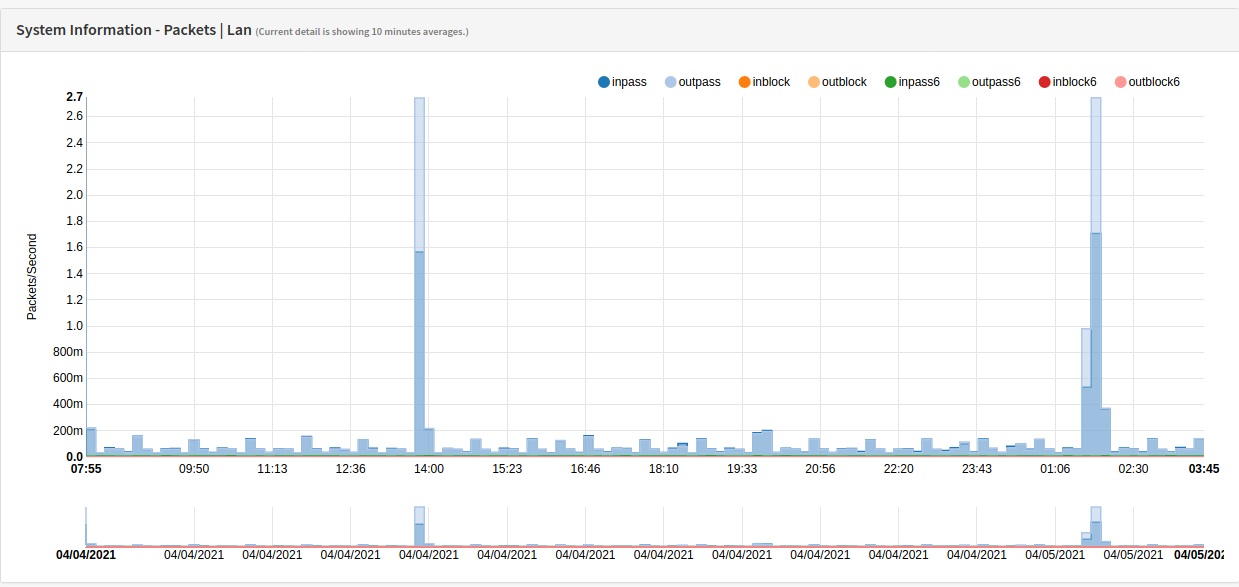
\includegraphics[width=0.7\textwidth]{Images/reporting/health_overview.PNG}
    \caption{Reporting - Healt}
    \label{opnsense:reporting_health}
\end{figure}

\subsection{NetFlow and Insight} \label{netflow}
NetFlow was created by Cisco and implemented in their equipment. There are different standards, but version 9\footnote{\url{https://www.ietf.org/rfc/rfc3954.txt}} is the newest one. Created by Darren Kerr and Barry Bruins in 1996 (\cite{CiscoSystemsDivisionInternetTechnologies2005}).

\warnblock{In the setup of NetFlow, version 9 is the default setting. \opnsense\ supports v5 and v9. The difference is: Version 5 = IPv4, version 9 = IPv4 and IPv6.}

It is possible to set up NetFlow to work internally or externally. In this case, we are setting it up to work internally. Follow the configuration below to start the collection of data:

\setupblock{\begin{enumerate}
    \item Goto \cmd{Reporting --> NetFlow}.
    \item Set:
    \begin{enumerate}
        \item \cmd{Listening interface} to \cmd{LAN and WAN}.
        \item \cmd{WAN interface} to \cmd{WAN}.
        \item Make a checkmark in \cmd{Capture local}.
        \item \cmd{Destination} to \cmd{127.0.0.1}.
    \end{enumerate}
    \item If you do not get any warnings, goto some web sites and create some traffic.
    \item Goto \cmd{Reporting --> Insight} and see if you get something similar to figure \ref{opnsense:reporting_insight}.
\end{enumerate}}



\begin{figure}[h!]
    \centering
    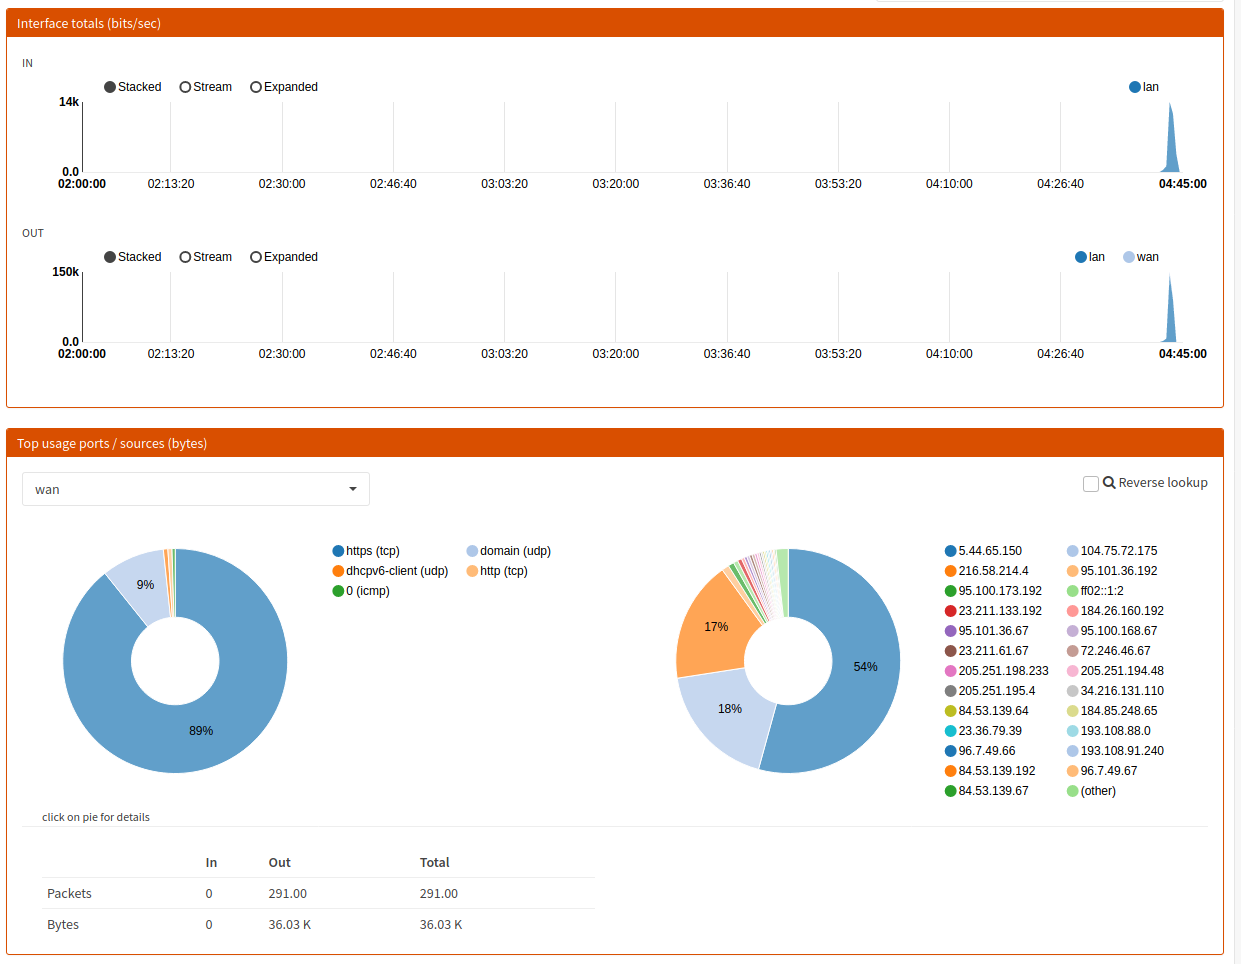
\includegraphics[width=0.7\textwidth]{Images/reporting/insight_report.PNG}
    \caption{Reporting - Insight}
    \label{opnsense:reporting_insight}
\end{figure}

\quesblock{\begin{enumerate}
    \item[49.] When is it useful to use an external NetFlow collector?
\end{enumerate}}

Detailed information from NetFlow can be exported, so it can be used else were. The exported data is in \cmd{.csv} form. Four different collections can be exported (Source address, source total, destination port, and interface totals.).

\quesblock{\begin{enumerate}
    \item[50.] Play around with the export function and see if you can find some opensource tool and import the data too.
\end{enumerate}}